\documentclass[conference]{IEEEtran}
\IEEEoverridecommandlockouts

\usepackage{cite}
\usepackage{amsmath,amssymb,amsfonts}
\usepackage{graphicx}
\usepackage{textcomp}
\usepackage{xcolor}
\usepackage{colortbl}
\usepackage{booktabs}
\usepackage{tikz}
\usepackage{pgfplots}
\pgfplotsset{compat=1.18}
\usetikzlibrary{arrows.meta,positioning,shapes.geometric,fit}
\definecolor{ctitle}{HTML}{2c2739}
\definecolor{mypurple}{HTML}{d2cce1}
\def\BibTeX{{\rm B\kern-.05em{\sc i\kern-.025em b}\kern-.08em
    T\kern-.1667em\lower.7ex\hbox{E}\kern-.125emX}}

\begin{document}

\title{From Ensemble and DistilBERT Baselines to Deep Metric Learning:\\
{\color{ctitle}An Extended Study for Imbalanced Windows PE Malware Detection}}

\author{\IEEEauthorblockN{Ly Ngoc Vu}
\IEEEauthorblockA{\textit{Industrial University of Ho Chi Minh City} \\
Ho Chi Minh City, Vietnam \\
dezzhuge@gmail.com}}

\maketitle

\begin{abstract}
Windows PE malware detection requires high recall under strict false-positive constraints, especially for imbalanced real-world data. This paper extends a prior ATC 2024 study that evaluated classical machine learning and text-based deep learning baselines. The extension introduces a deep metric learning (DML) branch on a shared Transformer backbone and compares five variants: baseline classification, ArcFace, Contrastive, Triplet, and Multi-Similarity. Evaluation uses multi-seed reporting and deployment-oriented metrics, including TPR@FPR operating points. Experimental results show that DML is beneficial but objective-dependent: Multi-Similarity provides the strongest overall operating profile, while ArcFace is unstable in strict low-FPR conditions despite high ranking metrics. The study provides practical guidance for objective selection in operational malware detection pipelines.
\end{abstract}

\begin{IEEEkeywords}
malware detection, PE files, deep metric learning, Transformer, low-FPR evaluation
\end{IEEEkeywords}

\section{\textcolor{ctitle}{Introduction}}
Malware detection on Windows PE files remains a high-impact cybersecurity task under evolving adversarial behavior and class-imbalanced data distributions \cite{sorel,bodmas}. Although modern classifiers often report high aggregate accuracy, real deployments are constrained by strict false-positive-rate (FPR) budgets, where threshold behavior is more informative than global metrics \cite{calibration,oodsecurity}. Prior results in the same project line showed that both optimized machine learning and text-based deep learning are strong baselines for PE classification \cite{atc2024}.

This paper extends that baseline study with deep metric learning (DML), motivated by the need for better class separation in highly imbalanced settings \cite{arcface,triplet,contrastive,msloss}. The central question is not whether DML can improve ranking metrics alone, but whether it improves low-FPR operational behavior.

The main contributions are:
\begin{enumerate}
\item A controlled objective-level comparison of baseline, ArcFace, Contrastive, Triplet, and Multi-Similarity on a shared Transformer backbone.
\item Multi-seed evaluation with deployment-oriented metrics, including TPR@FPR targets.
\item An operational analysis showing that objective choice materially affects low-FPR reliability.
\end{enumerate}

The remainder of this paper is organized as follows. Section II positions the extension relative to prior work. Section III summarizes the methodology and system design. Section IV presents experiments and results. Section V discusses implications and validity threats. Section VI concludes and outlines future work.

\section{\textcolor{ctitle}{Related Work and Extension Scope}}
\subsection{Prior ATC 2024 Results}
The prior paper reported:
\begin{enumerate}
\item Classical ML models: Logistic Regression, Random Forest, SVC, XGBoost, plus ensemble voting/stacking.
\item Text-based deep learning models: LSTM, BiLSTM, DistilBERT.
\item Large PE dataset setting (\textasciitilde34k samples) with high performance.
\end{enumerate}

\subsection{Extension in This Paper}
Recent metric-learning objectives, including ArcFace, Triplet, Contrastive, and Multi-Similarity, are widely adopted for discriminative embedding learning \cite{arcface,triplet,contrastive,msloss,dmlsurvey}. However, comparative evidence in PE malware settings under strict operating points is limited.

This work extends prior results by adding:
\begin{enumerate}
\item Objective-level study of DML variants.
\item Multi-seed statistical evaluation.
\item Deployment-oriented low-FPR analysis.
\end{enumerate}

\section{\textcolor{ctitle}{Methodology}}
A shared Transformer backbone is used, while objectives/heads vary:
\begin{enumerate}
\item baseline: cross-entropy/focal classification.
\item arcface: angular margin objective.
\item contrastive: pairwise distance objective + classification.
\item triplet: relative distance objective with hard mining.
\item multi\_similarity: weighted hard-pair similarity objective.
\end{enumerate}

\subsection{Experimental Setup}
The dataset setting follows the prior project pipeline and preserves the same PE text-feature processing strategy \cite{atc2024}. The extended pipeline evaluates five variants through a single runner and stores per-variant outputs for reproducibility. Model quality is assessed by Accuracy, Precision, Recall, F1, ROC-AUC, and PR-AUC. Operational reliability is measured with TPR@FPR points to reflect defender-oriented deployment constraints.

\subsection{LVModel Architecture Details}
The base LVModel is a Transformer encoder classifier implemented in Flax/JAX. Let input token IDs be
$\mathbf{X}\in\mathbb{N}^{B\times T}$, where $B$ is batch size and $T$ is sequence length (capped by $T\leq 380$ in the current setup).

\textbf{Embedding and positional encoding:}
\begin{equation}
\mathbf{H}_0 = E_{\text{tok}}(\mathbf{X}) + E_{\text{pos}}(1{:}T),
\end{equation}
where both embedding tables use normal initialization ($\sigma=0.02$).

\textbf{Shared MHA block implementation:}
for each encoder layer, a single dense projection computes concatenated QKV:
\begin{equation}
\mathrm{QKV} = W_{qkv}\mathbf{H}\in\mathbb{R}^{B\times T\times 3d},
\end{equation}
then reshaped to $(3,B,h,T,d_h)$ where $d_h=d/h$ and $h$ is head count.
Attention logits use scaled dot-product:
\begin{equation}
\mathbf{S} = \frac{\mathbf{Q}\mathbf{K}^{\top}}{\sqrt{d_h}},\quad
\mathbf{A}=\mathrm{softmax}(\mathbf{S}),
\end{equation}
followed by attention dropout and output projection back to $d$ dimensions.

\textbf{Encoder block design (pre-norm):}
each layer applies LayerNorm before attention and feed-forward modules:
\begin{align}
\tilde{\mathbf{H}} &= \mathrm{LN}(\mathbf{H}_{l-1}),\\
\mathbf{A} &= \mathrm{MHA}(\tilde{\mathbf{H}}), \quad
\mathbf{H}' = \mathbf{H}_{l-1} + \mathbf{A},\\
\mathbf{F} &= W_2\,\mathrm{Dropout}\!\left(\mathrm{GELU}\!\left(W_1\,\mathrm{LN}(\mathbf{H}')\right)\right),\\
\mathbf{H}_{l} &= \mathbf{H}' + \mathrm{Dropout}(\mathbf{F}).
\end{align}
This is a \textbf{pre-norm Transformer} with two residual paths (attention and FFN), improving optimization stability.

\textbf{Pooling and classification:}
the sequence representation is mean pooled and passed through a tanh pooler and LayerNorm classifier:
\begin{align}
\mathbf{z} &= \frac{1}{T}\sum_{t=1}^{T}\mathbf{H}_{L,t},\\
\mathbf{p} &= \tanh(W_p\mathbf{z}),\\
\mathbf{y} &= W_c\,\mathrm{LN}(\mathrm{Dropout}(\mathbf{p})).
\end{align}
In experiments, the instantiated architecture uses $d_{\text{model}}=256$, $h=8$, $d_{\text{ff}}=512$, and $L=2$.

\textbf{Metric-learning variants:}
ArcFace, Contrastive, Triplet, and Multi-Similarity share the same encoder trunk, then add an embedding projection
($d_{\text{emb}}=256$), LayerNorm, and $\ell_2$ normalization. The projected embedding is consumed by a task-specific head:
ArcFace angular-margin classifier, or linear logits with auxiliary metric losses (contrastive/triplet/MS).

\subsection{Pipeline Overview}
Figure~\ref{fig:pipeline} summarizes the end-to-end training and evaluation flow used for baseline and DML variants.
\begin{figure*}[!t]
\centering
\resizebox{\textwidth}{!}{%
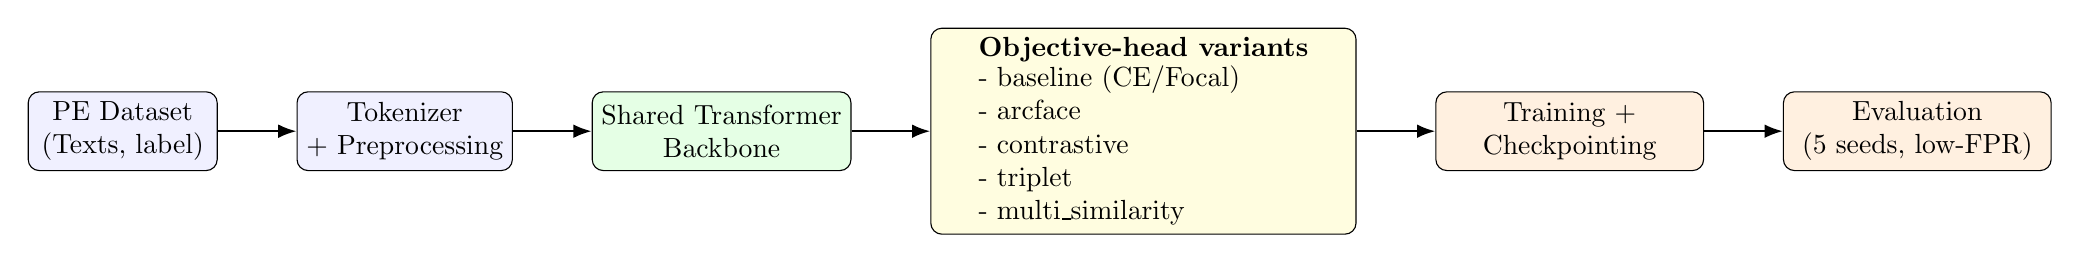
\begin{tikzpicture}[
    node distance=9mm and 10mm,
    stage/.style={draw, rounded corners, align=center, minimum height=10mm, minimum width=24mm, fill=blue!6},
    core/.style={draw, rounded corners, align=center, minimum height=10mm, minimum width=30mm, fill=green!10},
    block/.style={draw, rounded corners, align=left, minimum height=18mm, minimum width=54mm, fill=yellow!12},
    evalbox/.style={draw, rounded corners, align=center, minimum height=10mm, minimum width=34mm, fill=orange!12},
    arrow/.style={-Latex, thick}
]
    \node[stage] (data) {PE Dataset\\(Texts, label)};
    \node[stage, right=of data] (prep) {Tokenizer\\+ Preprocessing};
    \node[core, right=of prep] (backbone) {Shared Transformer\\Backbone};
    \node[block, right=of backbone] (heads) {\textbf{Objective-head variants}\\[-0.4mm]
        - baseline (CE/Focal)\\
        - arcface\\
        - contrastive\\
        - triplet\\
        - multi\_similarity};
    \node[evalbox, right=of heads] (train) {Training +\\Checkpointing};
    \node[evalbox, right=of train] (eval) {Evaluation\\(5 seeds, low-FPR)};

    \draw[arrow] (data) -- (prep);
    \draw[arrow] (prep) -- (backbone);
    \draw[arrow] (backbone) -- (heads);
    \draw[arrow] (heads) -- (train);
    \draw[arrow] (train) -- (eval);
\end{tikzpicture}}
\caption{Unified pipeline for baseline and DML variants.}
\label{fig:pipeline}
\end{figure*}

\section{\textcolor{ctitle}{Results}}
\subsection{Prior ATC 2024 Baselines}
\begin{table}[htbp]
\caption{ML baselines from prior paper}
\centering
\footnotesize
\begin{tabular}{lcccc}
\toprule
\rowcolor{mypurple!55}
Model & Precision & Recall & F1 & Accuracy \\
\midrule
Logistic Regression & 0.990086 & 0.990232 & 0.990111 & 0.990112 \\
Random Forest & 0.990000 & 0.990382 & 0.990402 & 0.990403 \\
SVC & 0.990000 & 0.988060 & 0.988075 & 0.988076 \\
XGBoost & 0.990000 & 0.991542 & 0.991566 & 0.991566 \\
\bottomrule
\end{tabular}
\label{tab:prior_ml}
\end{table}

\begin{table}[htbp]
\caption{Deep learning baselines from prior paper}
\centering
\footnotesize
\begin{tabular}{lcccc}
\toprule
\rowcolor{mypurple!55}
Model & Precision & Recall & F1 & Accuracy \\
\midrule
DistilBERT & 0.9864895 & 0.9865220 & 0.9864705 & 0.986471 \\
LSTM & 0.9674135 & 0.9674490 & 0.9674130 & 0.967413 \\
BiLSTM & 0.9507005 & 0.9499545 & 0.9500705 & 0.950102 \\
\bottomrule
\end{tabular}
\label{tab:prior_dl}
\end{table}

\subsection{New DML Results}
\begin{table}[htbp]
\caption{Aggregated 5-seed metrics (mean)}
\centering
\scriptsize
\setlength{\tabcolsep}{3pt}
\resizebox{\columnwidth}{!}{%
\begin{tabular}{lccccc}
\toprule
\rowcolor{mypurple!55}
Variant & Accuracy & F1 & ROC-AUC & PR-AUC & TPR@FPR=1e-2 \\
\midrule
baseline & 0.9924 & 0.9960 & 0.9983 & 0.9999 & 0.9754 \\
arcface & 0.7979 & 0.7934 & 0.9704 & 0.9984 & 0.0000 \\
contrastive & 0.9931 & 0.9964 & 0.9971 & 0.9997 & 0.9533 \\
triplet & 0.9932 & 0.9964 & 0.9969 & 0.9998 & 0.9351 \\
multi\_similarity & \textbf{0.9946} & \textbf{0.9972} & 0.9978 & 0.9999 & \textbf{0.9851} \\
\bottomrule
\end{tabular}
}
\label{tab:new_results}
\end{table}

\section{\textcolor{ctitle}{Discussion}}
The results indicate that DML is helpful but not uniformly so. Multi-Similarity yields the strongest overall profile, improving low-FPR sensitivity while maintaining top-tier F1 and accuracy. Baseline remains highly competitive, indicating a strong representation backbone and training recipe. ArcFace shows a notable mismatch between ranking quality and low-FPR behavior, suggesting sensitivity to margin-scale calibration under class imbalance.

Main findings:
\begin{enumerate}
\item DML helps, but improvements are objective-dependent.
\item Multi-Similarity is strongest overall in this setup.
\item Baseline remains highly competitive.
\item ArcFace requires further calibration/tuning for strict low-FPR deployment.
\end{enumerate}

\subsection{Threats to Validity}
\begin{enumerate}
\item \textbf{Single-domain evaluation}: results are derived from one PE data pipeline; broader cross-dataset validation is needed.
\item \textbf{Seed count}: five-seed reporting improves stability estimates but does not eliminate uncertainty.
\item \textbf{Calibration sensitivity}: thresholded performance may shift under temporal drift and distribution changes.
\item \textbf{Static-feature bias}: packed or heavily obfuscated binaries may require additional dynamic/contextual signals.
\end{enumerate}

\section{\textcolor{ctitle}{Conclusion}}
This extended study confirms that text-based PE malware detection can achieve high performance and that DML can further improve deployment-oriented behavior when the objective is carefully selected. Multi-Similarity is the recommended candidate in the current experiments.

\subsection*{Future Work}
Planned next steps include explicit calibration studies, statistical significance testing across objectives, cross-dataset generalization experiments, and robustness analysis under packing/obfuscation and temporal drift.

\section*{Acknowledgment}
This work extends the authors' prior ATC 2024 study and integrates new metric-learning experiments and analysis.

\begin{thebibliography}{00}
\bibitem{atc2024} L. N. Vu and D. T. Phuc, "Windows Malware Detection: Exploring from Machine Learning to Text-Based Deep Learning Approaches," in Proc. ATC, 2024.
\bibitem{arcface} J. Deng et al., "ArcFace: Additive Angular Margin Loss for Deep Face Recognition," CVPR, 2019.
\bibitem{msloss} X. Wang et al., "Multi-Similarity Loss with General Pair Weighting for Deep Metric Learning," CVPR, 2019.
\bibitem{triplet} F. Schroff et al., "FaceNet: A Unified Embedding for Face Recognition and Clustering," CVPR, 2015.
\bibitem{contrastive} R. Hadsell et al., "Dimensionality Reduction by Learning an Invariant Mapping," CVPR, 2006.
\bibitem{sorel} A. Harang and E. M. Rudd, "SOREL-20M: A Large Scale Benchmark Dataset for Malicious PE Detection," arXiv:2012.07634, 2020.
\bibitem{bodmas} BODMAS Dataset, "Benchmark for malware analysis at scale," 2021.
\bibitem{dmlsurvey} W. Zheng, J.-H. Lai, and P. C. Yuen, "A Survey on Deep Metric Learning: Approaches and Applications," arXiv:2303.15032, 2023.
\bibitem{calibration} C. Guo et al., "On Calibration of Modern Neural Networks," ICML, 2017.
\bibitem{oodsecurity} S. Wang et al., "A Comprehensive Survey of Out-of-Distribution Detection Methods for AI Security," ACM Comput. Surv., 2024.
\end{thebibliography}

\end{document}
